\documentclass[letterpaper,12pt,oneside]{book} %book

%\usepackage[a4paper,includeall,bindingoffset=0cm,margin=2cm,marginparsep=0cm,marginparwidth=0cm]{geometry}
\usepackage[top=1in, left=0.9in, right=1.25in, bottom=1in]{geometry}
%\usepackage{ThesisMartinIPN}
\usepackage[utf8]{inputenc}
\usepackage{url}
\usepackage[T1]{fontenc}
\usepackage[spanish,es-nodecimaldot,es-tabla]{babel}

% Poner imagenes juntitas
\usepackage{graphicx}
\usepackage{caption}
\usepackage{subcaption}

%\usepackage{graphicx}
\usepackage{tikz}
\usepackage{tocloft}
\graphicspath{{./figs/}}
\usepackage{setspace}
\usepackage{comment}
\usepackage{hyperref}

% Simbolos especiales 
\usepackage{amssymb, amsbsy}

\usepackage{amsmath} %Paquetes matemáticos de la American Mathematical Society

% Quitar la identación de los parrafos
\setlength\parindent{0pt}   

% Algoritmos
\usepackage[ruled,vlined]{algorithm2e}
\SetKwComment{Comment}{/* }{ */}


%Librerias nuevas. Poner número a lado del Chapter
\usepackage{titlesec, blindtext, color}
\definecolor{gray75}{gray}{0.75}
\newcommand{\hsp}{\hspace{20pt}}
\titleformat{\chapter}[hang]{\Huge\bfseries}{\thechapter\hsp\textcolor{gray75}{|}\hsp}{0pt}{\Huge\bfseries}

\usepackage{ragged2e}

% Quitar el heading
\usepackage{fancyhdr}            % Permits header customization. See header section below.
\fancypagestyle{plain}{
    \lhead{}
    \fancyhead[R]{}
    \fancyhead[L]{}
    \renewcommand{\headrulewidth}{0pt}
    
    \lfoot{}
    \fancyfoot[R]{\thepage}
    \fancyfoot[C]{}
    \fancyfoot[L]{}
    \renewcommand{\footrulewidth}{0pt}
}

\pagestyle{fancy}
\fancyhead[R]{}
\fancyhead[L]{}
\renewcommand{\headrulewidth}{0pt}

\fancyfoot[R]{\thepage}
\fancyfoot[C]{}
\fancyfoot[L]{}
\renewcommand{\footrulewidth}{0pt}


\urlstyle{same}
\hypersetup{
   colorlinks=true,
   urlcolor=cyan,
   linkcolor=black,
   citecolor=black,
   filecolor=magenta,
   pdftitle={Sharelatex Example},
   pdfpagemode=FullScreen,
}
\usepackage{cite}


\begin{document}



\begin{titlepage}
  \thispagestyle{empty}
  \begin{minipage}[c][0.17\textheight][c]{0.25\textwidth}
    \begin{center}
    \hspace*{-13mm}
      
\includegraphics[ height=5cm]{Images/logo-ipn.png}
    \end{center}
  \end{minipage}
  \begin{minipage}[c][0.195\textheight][t]{0.75\textwidth}
    \begin{center}
      \vspace{0.3cm}
             {\color{black}\textsc{\large Instituto Politécnico Nacional} }\\[0.5cm]
             \vspace{0.3cm}
                    {\color{black}\hrule height3pt}
                    \vspace{.2cm}
                           {\color{black}\hrule height2pt}
                           \vspace{.8cm}
                           \textsc{ \large Escuela Superior de Cómputo}\\[0cm] %
    \end{center}
  \end{minipage}
  \begin{minipage}[c][0.81\textheight][t]{0.25\textwidth}
    \vspace*{5mm}
    \begin{center}
      \hskip0.5mm
             \vspace{5mm}
             \hskip2pt
                 {\color{black}\vrule width3pt height13cm}
                 \hskip2mm
                     {\color{black}\vrule width1pt height13cm} \\
                     \vspace{5mm}
                     \hspace*{1mm}
                     
\includegraphics[height=4cm]{Images/escudoESCOM.png}
    \end{center}
  \end{minipage}
  \begin{minipage}[c][0.81\textheight][t]{0.75\textwidth}
    \begin{center}
      \vspace{1cm}

      {\color{black}{\large\scshape Semestre 2023-1}}\\[.2in]

      \vspace{0.5cm}            

      \textsc{\LARGE PRACTICA 5}\\[1.5cm]
      \textsc{\large Grupo: 3CV11}\\[0.5cm]
      \textsc{\large Materia: Análisis de Algoritmos}\\[0.5cm]
      
      {\color{black}\textsc{\large Alumnos:}}\\[0.5cm]
      \textsc{\large {Isaac Sánchez Verdiguel}}\\[1cm]
      \textsc{ {isanchezv1603@alumno.ipn.mx}}\\[1cm]   
      \textsc{\large {Axel Treviño Palacios}}\\[1cm]
      \textsc{ {atrevinop1500@alumno.ipn.mx}}\\[1cm]   
      
      
      
      \vspace{0.5cm}

      {\large\scshape 
        {\color{black}Maestro:}\\[0.3cm] {Benjamin Luna Benoso}}\\[.2in]

      \vspace{0.5cm}
       
      \large{21 Diciembre 2022}
    \end{center}
  \end{minipage}
\end{titlepage}
%---------------------------------
\tableofcontents
\listoffigures







\chapter{Introducción}



% Resumen
\section{Resumen}
    La práctica consta del análisis de complejidad de dos algoritmos iterativos y sus respectivas gráficas.

    \begin{description}
        \item [Python]
        \item [Algoritmo]
        \item [Complejidad]
    \end{description}

% La introducción a la práctica
\section{Introducción}
    Los algoritmos son una parte fundamental de la ciencia de la computación, ya que estos al ser computables pueden dar solución o una idea más concreta acerca de la solución de un problema.
    
    Un algoritmo no siempre dará una solución correcta, lo cual jamás será malo, porque esto nos ayudará a poder minimizar su radio de error. Una característica casi obligatoria para el buen funcionamiento de un algoritmo es su \textbf{rendimiento y eficacia}. El rendimiento adecuado se encuentra en la solución más rápida y menos costosa. \cite{Algorithm}
    
    La importancia de conocer el costo y las soluciones de un algoritmo es que sepamos si las respuestas dadas son las esperadas. Esto nos ayuda a resolver los problemas de manera concisa. (cita)
    
    Dentro de esta práctica, podremos ver dos algoritmos puestos a prueba de su complejidad temporal. Dando respuesta a sus diversas soluciones, desde las más eficientes hasta las que hacen que el algoritmo no pueda proporcionar las respuestas esperadas. 



\chapter{Desarrollo}

% Conceptos Básicos
\section{Conceptos Básicos}
    La \textbf{complejidad temporal}, dentro del análisis de algoritmos, es el número de operaciones que ejecuta un algoritmo en cierto tiempo. Su denotación es T(n) y puede ser analizada mediante dos tipos de análisis:
    
    \begin{itemize}
        \item Análisis de priori: entrega una función que muestra el tiempo de cálculo de un algoritmo.
        \item Análisis a posteriori: es la prueba en tiempo real del algoritmo, midiendo su costo mediante valores de entrada. 
    \end{itemize}
    
    El análisis de complejidad temporal define que un algoritmo alcanza su máximo potencial cuando los valores de entrada son mayores al tiempo estimado de ejecución, siendo que es factible poder completar sus ejecuciones en menor tiempo posible. 
    
    \textbf{Programación Dinámica} La programación dinámica es un proceso algorítmico que los informáticos y programadores emplean para abordar las dificultades de optimización. Cuando la programación dinámica se incorpora, el algoritmo utilizado para abordar problemas de codificación difíciles los descompone en subproblemas. Una solución optimizada para cada subcuestión puede entonces aplicarse a todo el escenario, dependiendo del tipo de solución que obtengan de cada subcuestión del código. Además, la programación dinámica optimiza la recursividad simple con las soluciones recursivas que los programadores obtienen mediante los cálculos de los subproblemas del problema \cite{ProDina}.

    \textbf{ Subsecuencia Común Más Larga} El problema de la subsecuencia común más larga (LCS) es encontrar la subsecuencia más larga presente en dos secuencias dadas en el mismo orden, es decir, encontrar la secuencia más larga que se puede obtener de la primera secuencia original eliminando algunos elementos y de la segunda secuencia original eliminando otros elementos \cite{Sub}.

    
    
    
\newpage
\section{Algoritmo LCS}
    \subsection{Algoritmo LCS}
   
    \subsubsection{Pseudocódigo Algoritmo LCS}
    El algoritmo lo realiza una comparación de dos archivos que contiene cada uno una cadena de caracteres en el cual se busca la Subsecuencia Común Más Larga (LCS) de forma que se llaman los archivos y se obtiene la sentencia, calculando de igual manera su longitud. Al ser llamada la función hace una comparación de longitudes para verificar que no sea cero (en caso de ser cero se retorna un cero), si existe una secuencia se acorta la misma eliminando el último elemento de la secuencia y repitiendo el proceso de forma recursiva, en caso contrario se encuentra el máximo de ambas y arroja el resultado.
        \begin{algorithm}
            \caption{LCS
            }\label{alg:two}
            \KwResult{$LCS$}
            
                % $d = 0$\;
                % $res = []$\;
                %print("Perfecto m: i") \;
                \eIf{len1 == 0 or len2 == 0}{
                    return 0\;
                }
                { 
                    \eIf{sec1[len1-1] == sec2[len2-1]}{
                        return 1 + lcs(sec1, sec2, len1-1, len2-1)\;
                    }
                    { 
                        return max(lcs(sec1, sec2, len1, len2-1), lcs(sec1, sec2, len1-1, len2))\;
                    }
                }
                % \For{$i\gets0$ \KwTo $len(diasTienda)$}{
                        
                % }

            
        \end{algorithm}
        
        
        
        
\chapter{Experimentación y Resultados}
    Aquí se presentaran los resultados del \textbf{Análisis a Priori y Posteriori} del algoritmo del granjero con Greedy
    
\section{Algoritmo: Granjero Greedy}
El algoritmo fue ejecutado en el lenguaje de programación \textbf{Python} en un entorno de \textbf{Linux}. A continuación se muestra el análisis de priori y posteriori. 
    \subsection{Análisis a Priori}
        La figura \ref{fig:priori} presenta el análisis a priori realizado sobre el pseudocódigo del algoritmo de Granjero de Greedy. Concluyendo que el algoritmo presenta \(T(n) = \theta(n)\)
        %\(f(n) = O(n)\)
        
        \begin{figure}[htp!]
            \centering
            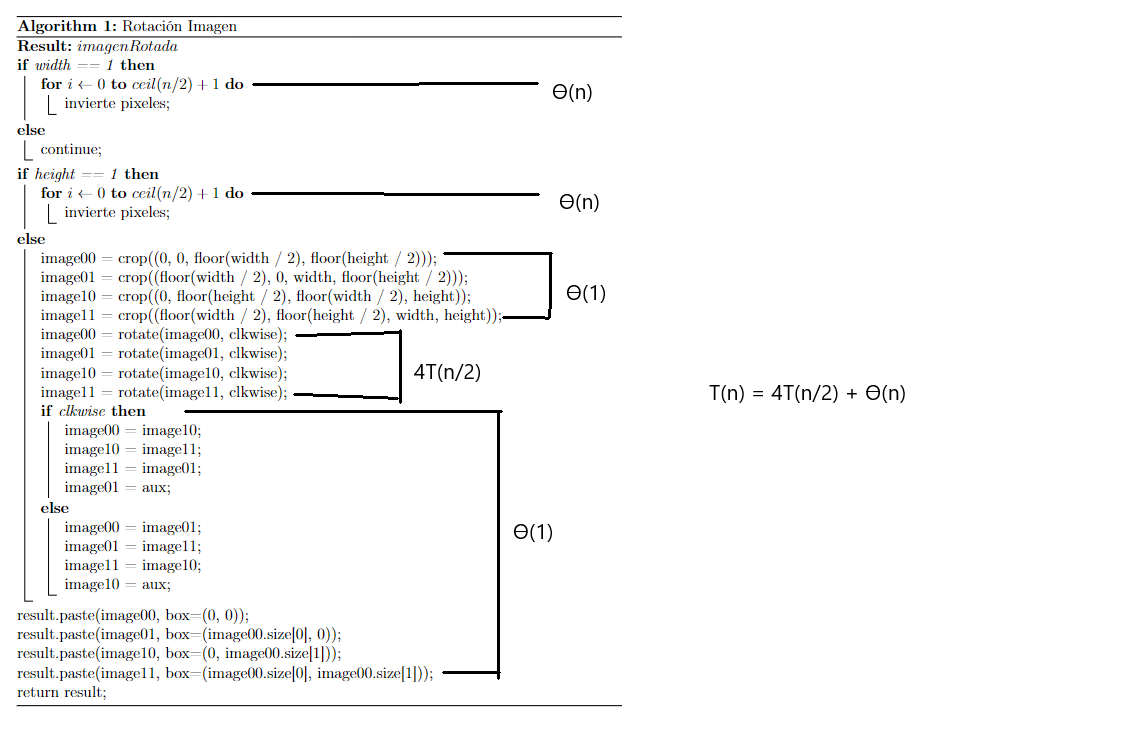
\includegraphics[width=0.5 \textwidth]{Images/A_Priori/priori.png}
            \caption{Análisis a Priori: Granjero Greedy}
            \label{fig:priori}
        \end{figure}
    
    \newpage    
    \subsection{Análisis a Posteriori}
        En el análisis posteriori se verifica que el análisis a priori demostró que la complejidad del peor caso es \(T(n) = \theta(n)\). En la figura \ref{fig:posteriori1} se muestra la función que acota al peor caso (línea verde) junto con los puntos que demuestran la complejidad del algoritmo funcionando de manera aleatoria.
        \begin{figure}[htp!]
            \centering
            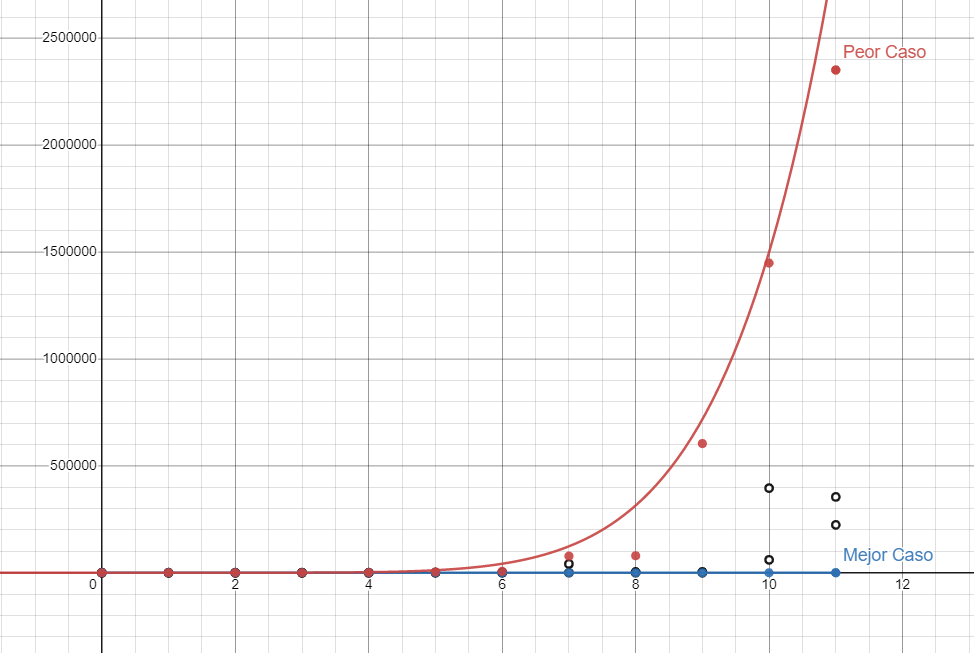
\includegraphics[width=1 \textwidth]{Images/A_Posteriori/posteriori.png}  
            \caption{Análisis a Posteriori: Granjero Greedy}
            \label{fig:posteriori1}
        \end{figure}
    
    
    
    \newpage
    \section{Pantallas de Ejecución del Algoritmo}
    Se muestra en la figura \ref{fig:terminal} la ejecución del algoritmo, demostrando la velocidad del algoritmo al ejecutar 200 casos.
    
        \begin{figure}[htp!]
            \centering
            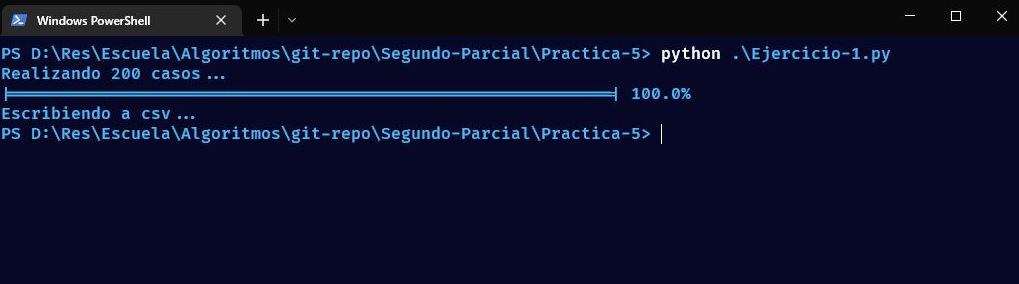
\includegraphics[width=0.8 \textwidth]{Images/Pantallas/terminal.png}  
            \caption{Ejecución de Granjero Greedy}
            \label{fig:terminal}
        \end{figure}
    
%\chapter{Avances}

% VACIOOOO
\chapter{Conclusiones}

\section{Conclusiones Generales}
    
    La técnica de Divide y Vencerás se torno difícil para nosotros a la hora de aplicarla al algoritmo propuesto para esta práctica. Repasamos los temas y vimos que nuestro punto bajo era la aplicación de funciones que no habíamos trabajado en el lenguaje Python. 

    Concluyendo que reforzar el tema de Divide y Vencerás no solamente ayuda al análisis de algoritmos sino que es un aprendizaje que se puede llevar a todos lados con su filosofía. 

\newpage
\section{Isaac Sánchez - Conclusiones}
    Esta práctica me resultó confusa, ya que la codificación del algoritmo para cambiar de posición las matrices de la imagen jamás lo había visto. Graias al aprendizaje de divide y vencerás pude entrar en detalle para poder lograrlo. Presentamos problemáticas de tiempo para concretar los problemas anexos. De ahí en fuera, fue una práctica que reforzó mis conocimientos.
    \begin{figure}[htp!]
            \centering
            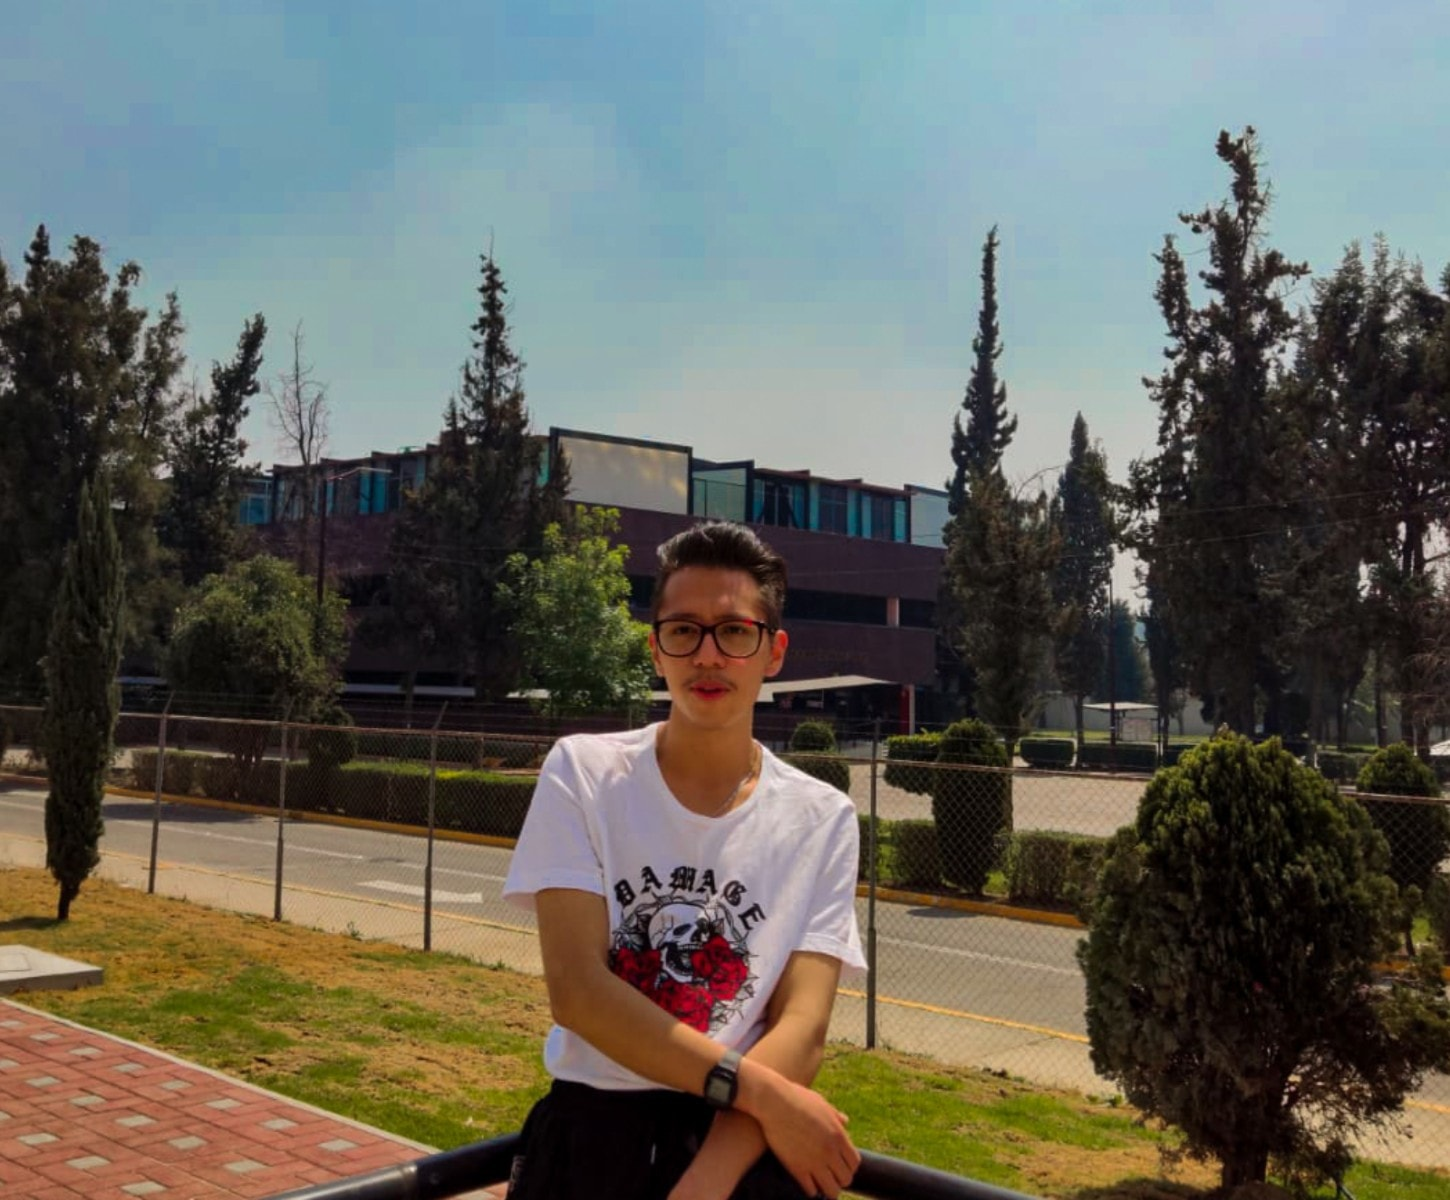
\includegraphics[width=1 \textwidth]{Images/Fotos_Alumnos/274612600_2528992867236334_6677874837890685705_n.jpg}  
            \caption{Isaac Sánchez}
            \label{fig:my_label1}
        \end{figure}
    


\newpage
\section{Axel Trevino - Conclusiones}
    Esta práctica es un buen ejemplo de los resultados de la recursividad adicionada al divide y vencerás, ya que cuando se piensa de manera normal, para rotar la imagen se tendrían que hacer dos cosas: cambiar los cuadrantes y rotarlos; pero al pensar que los cuatro cuadrantes igualmente son imágenes, sólo hay que aplicar el algoritmo ad infinitum y ya, todo se resuelve con el mismo proceso
    \begin{figure}[htp!]
            \centering
            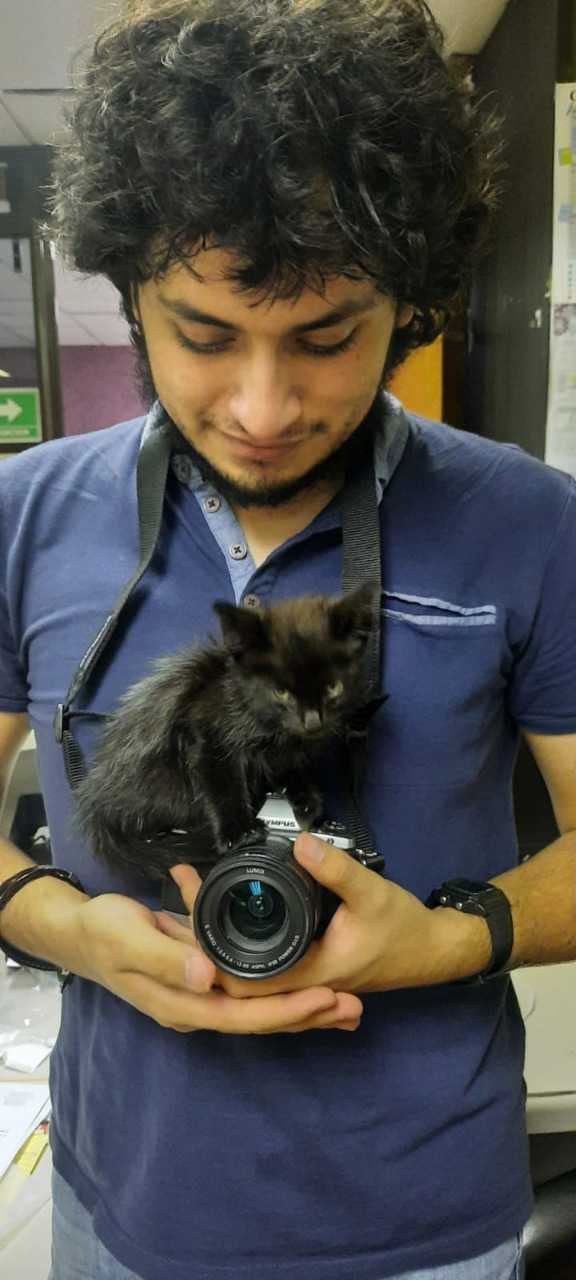
\includegraphics[width=0.4 \textwidth]{Images/Fotos_Alumnos/axel.jpg}  
            \caption{Axel Treviño}
            \label{fig:my_label2}
        \end{figure}

\chapter{Anexo}

    \section{Problemas y Ejercicios}
        En esta sección se aborda la solución de los problemas solicitados durante las clases previas a la práctica. 

        \subsection{Ejercicio 1}
            \textit{Descripción}: Contestar las siguientes preguntas.

            \begin{enumerate}
                \item Documentar el orden de complejidad de la mochila fraccionaria.
                \textbf{Respuesta:} El orden de complejidad de la mochila fraccionaria es \(\theta(n\log{n})\)
                \item Mostrar mediante un contraejemplo que en el caso de elegir objetos enteros, el algoritmo voraz propuesta para el caso fraccionario puede no generar soluciones óptimas.
                \textbf{Respuesta:} No funcionaría por el simple hecho de que un objeto entero no puede generar una solución de un valor entero. 
                \item ¿Cuál sería la mejor función de selección voraz en el caso en el que todos los objetos tuvieran el mismo valor?
                \textbf{Respuesta:} Se basaría en los valores más pequeños, al ser todos iguales algunos se queden fuera si la mochila queda sin espacio.
                \item ¿Cuál sería la mejor función de selección voraz en el caso en el que todos los objetos tuvieran el mismo peso?
                \textbf{Respuesta:} No afectaría ya que se mira por el valor y no por el peso. 
                
            \end{enumerate}
            
            

            

        \newpage
        \subsection{Ejercicio 2}
            \textit{Descripción}: Construir la codificación de Huffman para la cadena ciencias de la tierra.
            \newline
            En la figura \ref{fig:huffman1} se muestra el árbol construido por medio de una página web de la cadena Ciencias de la Tierra.
            \begin{figure}[htp!]
                \centering
                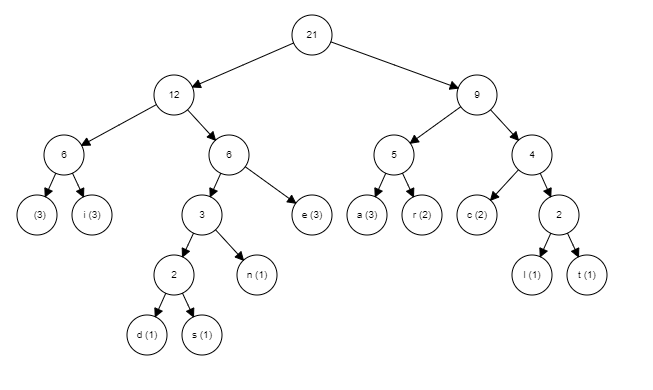
\includegraphics[width=0.7 \textwidth]{Images/HUFFMAN/HUFFMAN_CT.png}  
                \caption{Codificación cadena Ciencias de la Tierra}
                \label{fig:huffman1}
            \end{figure}
    
                
        \subsection{Ejercicio 3}
            \textit{Descripción}: Determinar el orden de complejidad el algoritmo de Huffman
            \newline
            La extracción de una cola de prioridad y al ser iterativo tiene una complejidad de \(O = n\log{n}\) 
            

        \subsection{Ejercicio 4}
            \textit{Descripción}: Documentar el orden de complejidad del algoritmo de Kruskal
            \newline
            Tiene una complejidad de \(O = n\log{n}\) Siendo n el número de vértices y a el número de aristas del grafo. Éste orden de complejidad es el obtenido al realizar la ordenación de las aristas de menor a mayor peso \cite{Kruskal}.
            
        \subsection{Ejercicio 5}
            \textit{Descripción}: Investigar el algoritmo de Prim
            \newline
            El algoritmo de Prim, dado un grafo conexo, no dirigido y ponderado, encuentra un árbol de expansión mínima. Es decir, es capaz de encontrar un subconjunto de las aristas que formen un árbol que incluya todos los vértices del grafo inicial, donde el peso total de las aristas del árbol es el mínimo posible.
            Después de realizar el análisis del código, tal y como muestran los costes indicados en el apartado anterior, se puede decir que, para el algoritmo de Prim, el orden de complejidad computacional temporal es de \(O(n^{2})\)). Siendo n el número de vértices del grafo \cite{Prim}.
                
        \subsection{Ejercicio 6}
            \textit{Descripción}: Documentar el orden de complejidad del algoritmo de Dijkstra.
            \newline
            El algoritmo de Dijkstra es un algoritmo eficiente de complejidad de \(O(n^{2})\) que sirve para encontrar el camino de coste mínimo desde un nodo origen a todos los demás nodos del grafo.
            


\bibliographystyle{apalike}
\bibliography{References/predoc.bib}




\end{document}
